\section{Case Studies}
\label{sec:resul}
Given that the framework makes several optimization algorithms available, the effectiveness of the framework is highly dependent on the effectiveness of these algorithms. This section focus on the evaluation of these algorithms on a series of computationally complex optimization problems within the architectural practice. This paper presents and evaluates two of those problems, a single- and a multi-objective optimization of simulation-based lighting and structural aspects of buildings.

When measuring the optimization algorithms' performance, several factors must be considered: (1) the optimization time is sensitive to the computational power of the machine where the algorithm is being run, (2) the non-determinism of several algorithms, and (3) the algorithms' hyperparameters. Firstly, to remove the time dependency of the machine characteristics and objective function's complexity, we measure the performance of the optimization algorithm in terms of the number of function evaluations, which is proportional to the actual time spent by the optimization process. Secondly, the stochastic nature of several optimization algorithms (e.g., random initial points, random modifications to solutions) might yield different results even when ran twice under the same configurations. To address this limitation, we run each stochastic algorithm three times and we use the average of the values to draw conclusions. Finally, for each problem, the algorithm's performance can be better or worse depending on its configurations. To this end, we opt for using the default algorithm's configurations, thus emulating the case when the architect's knowledge does not suffice to properly fine-tune the algorithm. 

All tests were run on a dual \textit{Intel Xeon CPU E5-2670 @ 2.60GHz with 64GB RAM}, where each daylight and structural simulation take approximately $7$ minutes and $40$ seconds to complete, respectively.

\subsection{Single-Objective Optimization: Ericeira House}
The first case study involved the optimization of the daylight conditions of a room in an isolated private house in Portugal~\cite{Caetano2018}. The room was designed with a set of façade shading panels that modulate the daylight conditions on the interior of the room. The panels are composed of a set of horizontal wood bars of different sizes, which alternate between one full-length bar and a set of smaller bars. For aesthetics reasons, the size and position of the smaller bars along the panel's width were randomized. The final pattern of the façade's shading panels was defined in terms of the length’s step, the maximum distance separating two consecutive bars, and the minimum and maximum lengths of the smaller bars. Initially, the goal was to find a solution for the shading panels that maximized the room's daylight performance, which was measured using the \ac{sUDI} metric \cite{Nabil2006}. While, in general, it is known that the more openings in the shading panels, the more daylight enter the room, this may also cause situations of uncomfortable glare. As a result, these situations should be accounted for, and, notwithstanding the values of the optimization process, architects should always perceive optimization results with a critical thinking. \Cref{fig:ericeira_multiple_panels} represents some design variations, ranging from denser patterns, with lower \ac{sUDI} values, to sparser ones, with higher \ac{sUDI} values.

\begin{figure}[htpb]
	\centering
	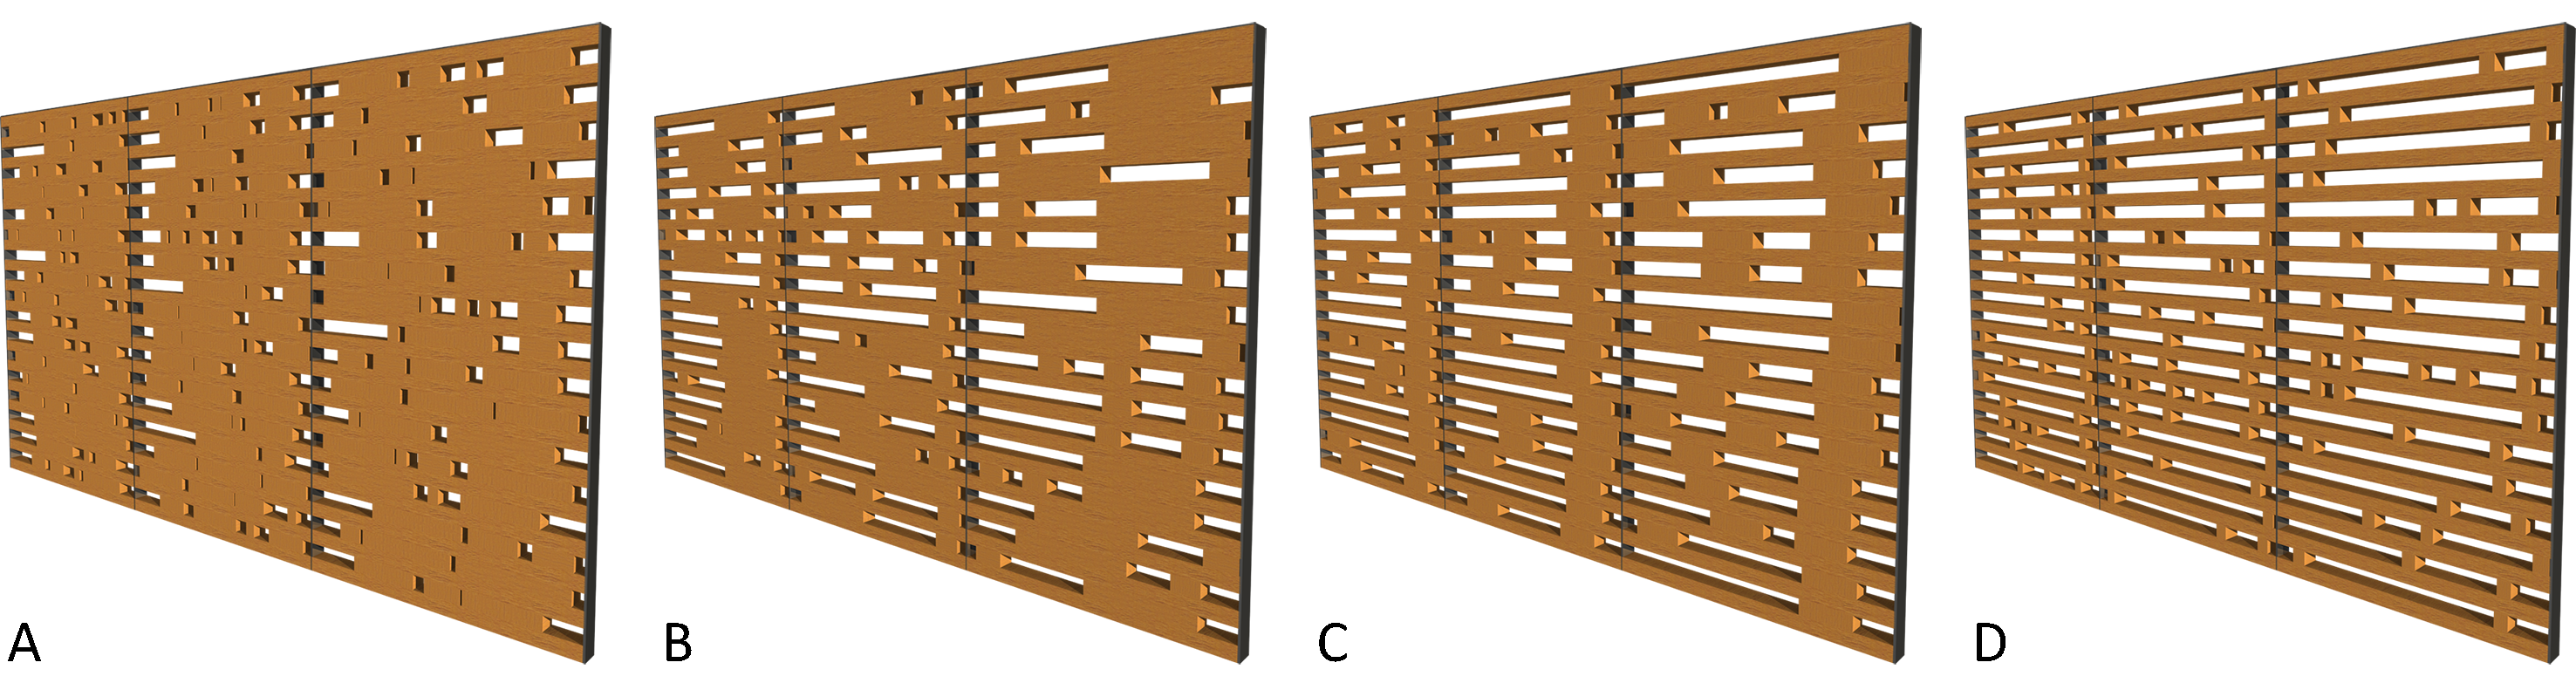
\includegraphics[width=\columnwidth]{../report/Images/Evaluation/Ericeira_2.png}
	\caption[Ericeira Solarium: Different representations of the shading panels’ geometric pattern]{Ericeira Solarium: Representation of the shading panels’ geometric pattern with different sUDI values (from left to right, 7\%, 62\%, 90\%, and 100\%).}
	\label{fig:ericeira_multiple_panels}
\end{figure}

Initially, we pursued a simple experimental approach to address this optimization problem \cite{Caetano2018}. To generate the design variants to evaluate, we used the \textit{Monte Carlo} and the \textit{Latin Hypercube sampling} algorithms. This approach allowed us to exploit previous knowledge about the shading panels and its impact on the daylight conditions of the room (e.g., that sparser patterns increase daylight performance) and, consequently, to produce a more efficient optimization process. In fact, based on this knowledge, we set several iterations of the different sampling methods and, within each iteration, we have further restrained the variables' to vary in smaller ranges, thus enforcing the sampling of incrementally more efficient designs. %\Cref{fig:ericeira_doe} shows an example of the results obtained during this process, as well as the solutions that were presented to the architects, so that they would choose the one that better suited their intentions.

Despite achieving optimal solutions with values of \ac{sUDI} of $100\%$, we have only achieved these solutions after $200$ function evaluations. Because each evaluation took approximately $7$ minutes to complete on a dual \textit{Intel Xeon CPU E5-2670 @ 2.60GHz with 64GB RAM}, the optimal solution was only obtained after $1400$ minutes, or, equivalently, $23.33$ hours. This large time complexity resulted from the fact that approaches based on sampling algorithms consist on the consecutive uninformed experimentation of multiple designs, i.e., without taking into consideration previous design evaluations, often evaluating irrelevant design solutions. Moreover, this approach required several manual interventions (e.g., analyse the results, redefine the variables' bounds, select number of evaluations). In an attempt to minimize the time complexity of the optimization process and to verify the impact of more guided approaches in \ac{BPO} problems, we have also tackled this problem using a \ac{SOO} approach \cite{Belem2018optimizeddesign}. Particularly, we evaluated the performance of $13$ different derivative-free optimization algorithms: $5$ direct-search, $3$ metaheuristics, and $5$ model-based. Given the time complexity of each function evaluation, we set a limit of $60$ function evaluations per run.

%http://papers.cumincad.org/data/works/att/caadria2018\_278.pdf
\begin{table}[htbp]
	\centering
	\caption[Ericeira Solarium: Mean best results and evaluations discriminated per algorithm]{Ericeira Solarium: Table with the mean best daylight results and mean evaluations to reach optimal solutions of each algorithm. Results are averaged over $3$ runs, each with $60$ evaluations.}
	\label{table:phase1results}
	\includegraphics[width=\textwidth]{../report/tables_and_code/Ericeira_phase1_stats_v1.pdf}
\end{table}

\Cref{table:phase1results} shows the mean best results and the standard deviation of the three runs, discriminated by algorithm. According to the results, in average, the global model-based algorithms \textit{\ac{GPR}}, \textit{\ac{RBF}CC}, and \textit{\ac{RBF}CL} were able to find an optimal solution within the first $30$ evaluations. Conversely, the local model-based algorithms \textit{\ac{COBYLA}} and \textit{\ac{BOBYQA}} performed rather poorly in this problem, converging to far from optimal solutions after $29$ and $48$ function evaluations, respectively. Regarding direct-search algorithms, the global algorithm \textit{\ac{DIRECT}} was able to find a close to optimal solution (with an \ac{sUDI} value of $98\%$) in the last function evaluation. Its local variant, \textit{\ac{DIRECT}-L}, and the local direct-search algorithms \textit{\ac{PRAXIS}} and \textit{SUBPLEX} fell short of the expected and barely managed to improve over $80\%$. Nevertheless, the simplex-based direct-search algorithm \textit{\ac{NMS}} performed surprisingly well, having achieved an average result of $89.67\%$ within the first $15$ evaluations. Finally, although metaheuristics performed better than most local model-based and direct-search algorithms, they seem to stagnate in design solutions with \ac{sUDI} values below the $88\%$, after $30$ evaluations.

\Cref{fig:phase1results} shows the average performance per algorithm class, also separating them in local or global algorithms. Overall, local algorithms seem to perform worse than all other algorithms, with local direct-search and model-based algorithms stagnating towards design solutions with \ac{sUDI} values below $75\%$ and $70\%$, respectively. Contrastingly, global algorithms were able to find design solutions with values of \ac{sUDI} larger than $80\%$. Despite the good initial performance of metaheuristics algorithms for the first $20$ evaluations, global direct-search algorithms quickly surpassed them, achieving close to optimal solutions with \ac{sUDI} values of $90\%$. Lastly, global model-based algorithms were, on average, the best performing algorithms, achieving close to optimal solutions shortly after $24$ evaluations. 

\begin{figure}[htbp]
	\centering
	\includegraphics[width=1\textwidth]{../report/Images/Evaluation/Ericeira_results_ph1_per_class.PNG}
	\caption[Ericeira Solarium: Mean best daylight results in function of the number of evaluations, discriminated per class of algorithms]{Ericeira Solarium: Mean best daylight results in function of the number of evaluations, discriminated per class of algorithms.}
	\label{fig:phase1results}
\end{figure}

Given the overall bad performance of local algorithms, we decided to assess their performance when initialized with different solutions. Notwithstanding their ability to quickly converge to locally optimal solutions, the quality of the found solutions highly depends on the solution used to initialize the search. Therefore, we have also studied the impact of different initial solutions in the performance of these algorithms. To this end, we tested all $5$ local algorithms with two different initial solutions: a bad solution, with a $7\%$ value of \ac{sUDI}, and a reasonable solution with a $78\%$ value of \ac{sUDI}. Moreover, we decided to further restrict the number of evaluations to $15$, thus emulating an hypothetical scenario, where users lack knowledge about different optimization algorithms and opt for testing several of them. Ideally, this would allow them to infer the most promising algorithm and obtain a reasonable solution to hot-start other algorithms and, potentially, improve the overall optimization time.

\Cref{fig:phase2results} presents the mean best daylight results found by each local optimization algorithm. As expected, no local algorithm was able to obtain a good solution when provided with a bad starting solution. On the one hand, when provided with a mild initial design, both \textit{\ac{COBYLA}} and \textit{\ac{NMS}} found the best designs achieving a \ac{sUDI} value of $99\%$. On the contrary, \textit{\ac{PRAXIS}} found the worse, and showed no relevant improvement over the initial design. Nevertheless, it initially managed to outperform other methods, achieving values of \ac{sUDI} of $80\%$. After $8$ evaluations, \textit{\ac{COBYLA}} and \textit{\ac{NMS}} quickly converged to near optimal designs, with \ac{sUDI} values of $99\%$ and $98\%$, respectively. \textit{\ac{BOBYQA}} and \textit{SUBPLEX} struggled to improve from the initial design.
\begin{figure}[htbp]
	\centering
	\includegraphics[width=\textwidth]{../report/Images/Evaluation/Ericeira_results_ph2.PNG}
	\caption[Ericeira Solarium: Mean best results of daylight performance in function of the number of evaluations, discriminated per local algorithm]{Ericeira Solarium: Mean best results daylight results as a function of the number of function evaluations, discriminated per local algorithm. Algorithms suffixed with \textit{HS} are given an initial solution with an \ac{sUDI} value of $78\%$, whilst algorithms suffixed with \textit{BS} are given an initial solution with an \ac{sUDI} value of $7\%$.}
	\label{fig:phase2results}
\end{figure}

On the other hand, when provided with a bad initial design, the best daylight result has an \ac{sUDI} value of $15\%$ and was found by \textit{\ac{NMS}} after $9$ evaluations. \textit{\ac{NMS}}, \textit{\ac{COBYLA}}, and \textit{SUBPLEX} exhibit similar performance, stagnating in a design with an \ac{sUDI} value of $11\%$ after $3$ evaluations, with \textit{\ac{NMS}} being able to further improve the design after $5$ evaluations. \textit{\ac{PRAXIS}} exhibits the worst performance among all methods, showing no significant improvements throughout the whole optimization process.


\subsection{Multi-Objective Optimization: Space Frame Optimization}
In this section, we evaluate two \ac{MOO} problems \cite{Belem2019MOO,IP2019MOO}. As previously discussed in \cref{ssec:performance}, addressing these problems comprises a difficult task, not only because of the higher complexity of the obtained results, but also because of the absence of standards regarding the best way to evaluate the \acp{MOOA}' performance. For these reasons, in this dissertation, we opted for evaluating the algorithms' performance in terms of the results returned by each algorithm, i.e., the \acp{aPF}. For each algorithm, we compute different indicators that measure the \acp{aPF} in terms of their cardinality, diversity, and accuracy.%: \ac{ONVGR}, \ac{ER}, Spacing, Maximum Spread, \ac{MPFE}, \ac{GD}, and \ac{HV}. 

Although some indicators measure aspects based exclusively on the \acp{aPF}, others require a reference set to compare with the \acp{aPF}. Ideally, this reference set would represent the real optimal solutions for the specified problem. Unfortunately, this set of optimal solutions, also called \ac{tPF}, is not known for most \ac{BPO} problems. In an attempt to better approximate it, we compute a fictitious Pareto Front, the \ac{cPF}, composed of the best solutions found by each algorithm. 

Note, however, that we aimed at measuring the average performance of each algorithm regarding an unknown \ac{tPF}. In general, computing an accurate approximation of the \ac{tPF} would require running the algorithms for thousands of iterations, which is not feasible in most \ac{BPO} problems involving time-consuming evaluation functions. As a consequence, we adopted a methodology similar to the one used in \cref{ssec:soocasestudy}, which quantifies the performance of each algorithm in terms of the mean value of three runs, using as reference, for each run, the corresponding \acp{cPF}. 

In the next sections, we present and discuss the obtained results for each algorithm. In \cref{appendix:appendixB}, we provide additional information about each algorithm's configuration and present the Pareto front plots corresponding to each run.

\subsubsection{Space Frame Optimization}
Motivated by the interest of architects in performing structural analysis \cite{Cichocka2017SURVEY}, the first \ac{MOO} case study consisted in the optimization of both the structural behavior and an \textit{ad-hoc} measure of the irregularity of an arc-shaped space frame. To instil irregularities in the space frame, we introduced three attractors that cause a deformation in the shape of the truss, each of which is defined in terms of its fixed-radius cylindrical coordinates in the arc-shaped space frame~\cite{Belem2019MOO}. To measure the goals for each design variant, we used (1) the Robot analysis tool to compute the maximum displacement of the structure, and (2) the sum of the Euclidean distances between the attractors. To increase the interest of this case study, we set out to minimize both objectives, thus promoting the conflict between them: placing the attractors near each other will weaken the structure and, thus, increase the maximum displacement of the space frame. In fact, to reduce the maximum displacement, the attractors should be scattered across the space frame but this implies larger distances among the three attractors, thus worsening the second objective. \Cref{fig:spaceframe} illustrates three examples of the space frame structure. 
\begin{figure}[htbp]
	\centering
	\includegraphics[width=1\textwidth]{../report/Images/Evaluation/truss-kat-small.png}
	\caption[Space Frame: Representation of three space frame design variants]{Space Frame: Representation of three design variations of the arc-shaped space frame, with copper balls representing the three attractors.}
	\label{fig:spaceframe}
\end{figure}

To optimize the space frame, we decided to test $10$ metaheuristics and $9$ model-based algorithms. On the one hand, each metaheuristic algorithm comprised a total of $15$ individuals/particles per iteration, which were evolved for $15$ iterations. On the other hand, model-based algorithms derived $100$ initial samples using the Latin Hypercube sampling algorithm, which were then used to create the initial approximation to the expensive evaluation function, upon which another $125$ evaluations were completed. Overall, every algorithm was limited to a total of $225$ function evaluations, each taking approximately $40$ seconds to complete on a dual \textit{Intel Xeon CPU E5-2670 @ 2.60GHz with 64GB RAM}. In total, each run is composed of $4275$ candidate solutions and takes approximately $2$ days to complete.

\Cref{table:spaceframe,table:spaceframestd} show the mean results of the performance indicators and corresponding standard deviations for the three runs, discriminated by the algorithms' classes and subclasses. As previously mentioned, we computed several performance indicators for each \ac{aPF}, which provide information about: (1) cardinality, measured by \ac{ONVGR} and \ac{ER}; (2) diversity, measured with Spacing and Maximum Spread; and (3) accuracy/convergence, measured with \ac{MPFE} and \ac{GD}. Moreover, we used a Pareto-compliant indicator, the \ac{HV}, to obtain a combined measure of all the three mentioned aspects. % To simplify the performance comparison among the different algorithms, we restrained the set of indicators to the unary ones. 
% 1 - Two set coverage não ia dar medidas relevantes porque raramente as diferentes frentes se tocam. 
% 2 - Epsilon indicators poderia ser interessante, mas não foi testada a implementação
% 3 - R-metrics requer funções de utilidade que não temos e que requer alguma sensibilidade em relação ao problema...

% The overall cardinality of each combined Pareto front is 14, 24, and 19, respectively.
When considering the cardinality aspect, the \ac{ONVGR} column of \cref{table:spaceframe} presents the ratio of optimal solutions between \acp{aPF} and \acp{cPF}. In general, metaheuristics seem to retrieve the most nondominated solutions within each run, whereas model-based algorithms seem to retrieve the least. In fact, among the model-based algorithms, the algorithms exploring random search strategies, i.e., the algorithms suffixed with \textit{Random}, yield fewer nondominated solutions, which may result from a poor exploration of the solution space. On average, the best performing algorithm, \textit{PAES}, is able to find twice the number of solutions that compose each \ac{cPF}, whereas model-based algorithms, including \textit{GPR+Random} and \acp{MLP} algorithms, struggled to find a set of optimal solutions with at least half of the size of the \acp{cPF}. 
%http://papers.cumincad.org/data/works/att/caadria2018\_278.pdf
\begin{table}[h!]
	\centering
	\caption[Space Frame: Mean values for the performance indicators results, discriminated per algorithms]{Space Frame: Mean values for the performance indicators results, discriminated by algorithm. Results are averaged over $3$ runs, each with $225$ evaluations.}
	\label{table:spaceframe}
	\includegraphics[width=\textwidth]{../report/Images/Evaluation/caadria/Results_Mean_20190428.PNG}
\end{table}

While the \ac{ONVGR} indicator provides an intuition about the richness of each algorithm's \acp{aPF}, many of the identified solutions might not be truly optimal, i.e., despite being optimal among all the evaluated solutions, these solutions might not belong to the corresponding \ac{cPF}. To this end, \ac{ER} is used to measure the percentage of false-optimal solutions for each algorithm. In this case, it becomes clear that even though \textit{PAES} retrieves twice as many optimal solutions as the \acp{cPF}, most of them are not truly optimal. Moreover, none of the solutions found by the $\epsilon$\textit{-MOEA}, \textit{MOEA/D}, and \textit{CMA-ES} metaheuristics algorithms belong to the \acp{cPF}. The same happens with some of the model-based algorithms, particularly, \textit{GPR+NSGA-II}, \textit{GPR+Random}, and \textit{MLP+Random}. On the other hand, \ac{PSO}-based metaheuristics algorithms, \textit{SMPSO} and \textit{OMOPSO}, exhibit the lowest \ac{ER} value, having found at least one optimal solution in each run.

The diversity aspect consists in the analysis of the distribution of the nondominated solutions across the objective space. The Spacing indicator measures the uniformity of the \acp{aPF}, regardless of the \acp{cPF}. Considering this indicator, the two \ac{ES} metaheuristic algorithms, \textit{PAES} and \textit{CMA-ES}, and one \ac{EA}-based metaheuristic algorithm, $\epsilon$\textit{-MOEA}, achieved the most uniform \acp{aPF}. Conversely, model-based algorithms seem to yield more irregular \acp{aPF}, namely, \textit{MLP+NSGA-II} and \textit{MLP+SMPSO} achieved the worst values of the Spacing indicator. Note, however, that this indicator merely provides an idea of the regularity of distribution of the solutions. Ideally, this indicator would also suggest a good coverage of the \ac{cPF}, i.e., that the \acp{aPF} found by each algorithm cover the same regions as the \acp{cPF}, instead of focusing on narrower regions. However, most of the algorithms that present the best Spacing scores achieve such values because most of the identified optimal solutions lie within the same small region but present a more uniform distribution. Besides this limitation, these indicators are also highly sensitive to outliers and to the number of retrieved solutions. % number of solutions also indirectly contributes to these scores of each indicators, since these indicators measure the distances between consecutive optimal solutions and the weight each outlier has in smaller or larger sets can greatly influence the final result.

Besides having an uniform distribution, when applicable, good Pareto fronts should also cover large extents of the objective space in order to provide more relevant trade-offs. \textit{Max Spread} measures the extent of the \acp{aPF} retrieved by each algorithm. On average, \textit{SMPSO}, \textit{GDE3}, and \textit{OMOPSO} are able to explore wider extents of the objective space. Observing \cref{table:spaceframe}, we conclude that, on average, \textit{SMPSO}, \textit{GDE3}, and \textit{OMOPSO} were able to cover the objective space better. Contrastingly, the \ac{ES}-based algorithms were the worst algorithms in this aspect, having explored smaller regions of the objective space. Regarding model-based algorithms, it is possible to observe that the ones based on \textit{SMPSO} were able to explore broader regions of the objective space than the ones based on \textit{NSGA-II} or \textit{Random} strategies. 
\begin{table}[]
	\centering
	\caption[Space Frame: Standard deviation values for the performance indicators results, discriminated by each algorithm]{Space Frame: Standard deviation values for the performance indicators results, discriminated by algorithm. Results are averaged over $3$ runs, each with $225$ evaluations.}
	\label{table:spaceframestd}
	\includegraphics[width=\textwidth]{../report/Images/Evaluation/caadria/Results_Std_20190428.PNG}
\end{table}

Another important aspect of \acp{aPF} is their accuracy and how close their solutions are from the \acp{cPF}. In this case study, we considered two accuracy indicators, \ac{MPFE} and \ac{GD}. On average, when considering \ac{MPFE}, every model-based algorithm retrieved \acp{aPF} whose \ac{MPFE} values were always better than the ones obtained by any metaheuristic. In particular, \textit{MLP+NSGA-II} and \textit{MLP+Random} have the smallest maximum error which means that all the points are at most at that distance from an optimal solution. Furthermore, the algorithms exploring a larger extent of the objective space, i.e., with higher values of Max Spread, have worse \ac{MPFE} values. This can be explained due to the lack of information about the \ac{tPF}, which is only being approximated by the best solutions found in each run, i.e., the \acp{cPF}. 

Notwithstanding the fact that \ac{MPFE} provides an estimate of the maximum error of the algorithms' \acp{aPF}, this indicator does not provide a real measure of how close the results are to the \acp{cPF}. To this end, we use the \ac{GD} indicator, which measures the average approximation of the \acp{aPF} retrieved by each algorithm to the closest solutions in the corresponding \acp{cPF}. \Cref{table:spaceframe} shows that, on average, \textit{MLP+NSGA-II} and \textit{PAES} present the best convergence towards the \ac{cPF}, and that \textit{GDE3} and \textit{OMOPSO} present the worst convergence values. These can be explained by the number of the nondominated solutions retrieved by each algorithm, as well as by the creation of clusters of optimal solutions near the \acp{cPF} that were discovered by \textit{PAES} and \textit{MOEA/D}, as is visible in \cref{sec:spaceframeoptimizationextra}. In general, other model-based algorithms also present reasonable scores, like the \textit{MLP+Random} or all the \ac{RF}-based algorithms even surpassing many metaheuristics algorithms, including \textit{CMA-ES}, $\epsilon$\textit{-MOEA}, \textit{NSGA-II}, and \textit{SPEA2}, thus suggesting better approximations.

In the end, we also used the \ac{HV} indicator, as it appraises the quality of a Pareto front with regards to all three aspects simultaneously. The best performing algorithms were the \ac{PSO}-based algorithms, \textit{SMPSO} and \textit{OMOPSO}, followed by \textit{GDE3}. Surprisingly, the \ac{PSO} model-based algorithms also present a good performance, when compared to other metaheuristics, and even to other model-based algorithms that explore \textit{Random} or \ac{EA} strategies to search for optimal solutions. Conversely, the worst performing algorithms were the \ac{ES}-based ones, \textit{CMA-ES} and \textit{PAES}, followed by \textit{GPR+Random}. % Finally, comparing different algorithms regarding \ac{IGD}, the \ac{PSO}-based metaheuristic algorithms still yielded the best results, whilst \ac{ES}-based metaheuristic algorithms yielded the worst. However, \textit{MOEA/D} unexpectedly reveals itself as the third best performing algorithm when considering the \ac{IGD} indicator. Although this seems odd, this value can be explained by the difference in the scales of both axis and to the higher density of Pareto optimal solutions in the $x$-axis for values between $1.2$ and $1.3$.
\begin{figure}[hptb]
	\centering
	\includegraphics[width=\textwidth]{../report/Images/Evaluation/caadria/All_Algorithms_all_runs-2019-04-13_1000dpi.png}
	\caption[Space Frame: Pareto front plot]{Space Frame: Algorithms' \acp{aPF} measuring the attractors distance, in function of the maximum displacement. These fronts are obtained by combining the values of the $3$ runs for each algorithm. The \ac{cPF} is formed by finding the nondominated solutions from all the evaluated solutions.}
	\label{fig:allruns}
\end{figure}

Overall, no single algorithm was able to outperform the others in terms of all the indicators. Nevertheless, the \ac{PSO}-based metaheuristics algorithms, \textit{OMOPSO} and \textit{SMPSO}, exhibited the overall best performance. Moreover, even though none of the model-based algorithms was able to surpass the \textit{SMPSO} and \textit{OMOPSO}, the model-based algorithms that use \textit{SMPSO} also exhibited a reasonable performance, better than several well-known metaheuristics, including $\epsilon$\textit{-MOEA}, \textit{MOEA/D}, \textit{CMA-ES}, and \textit{SPEA2}. \Cref{fig:allruns} presents a combined view of all the algorithms for every run, where it is possible to visualize the extent of \ac{PSO}-based algorithms and the high density region to which several \acp{EA} and \acp{ES} algorithms converged.
